\documentclass[11pt,english,a4paper]{article}

\usepackage[utf8]{inputenc}          % Allows UTF-8 encoded characters in the .tex-file.
\usepackage{babel,csquotes,textcomp} % Set LaTeX to structure the content following international academic standards.
\usepackage[titletoc,toc]{appendix}
\usepackage{subfig}

\usepackage{hyperref}
\usepackage{graphicx}
\usepackage{pdfpages}
\usepackage{listings}
\usepackage{wrapfig}
\usepackage{color,colortbl}
\usepackage{lettrine}
\usepackage[font={small,it}]{caption}
\usepackage{multirow}
\usepackage{tabularx}
\usepackage{footnote}
\usepackage{enumitem}
\usepackage{amsmath}

\usepackage[
    backend=biber,
    style=numeric
]{biblatex}
\addbibresource{refs.bib}

\lstset{ %
  basicstyle=\ttfamily\small,     
  backgroundcolor=\color{white},   % choose the background color
  breaklines=true,                 % automatic line breaking only at whitespace
  captionpos=b,                    % sets the caption-position to bottom
  commentstyle=\color{mygreen},    % comment style
  escapeinside={\%*}{*)},          % if you want to add LaTeX within your code
  keywordstyle=\color{blue},       % keyword style
  stringstyle=\color{mymauve},     % string literal style
}

\title{Lab report \\ GPSDO}
\author{Aril Schultzen}

\begin{document}
\maketitle
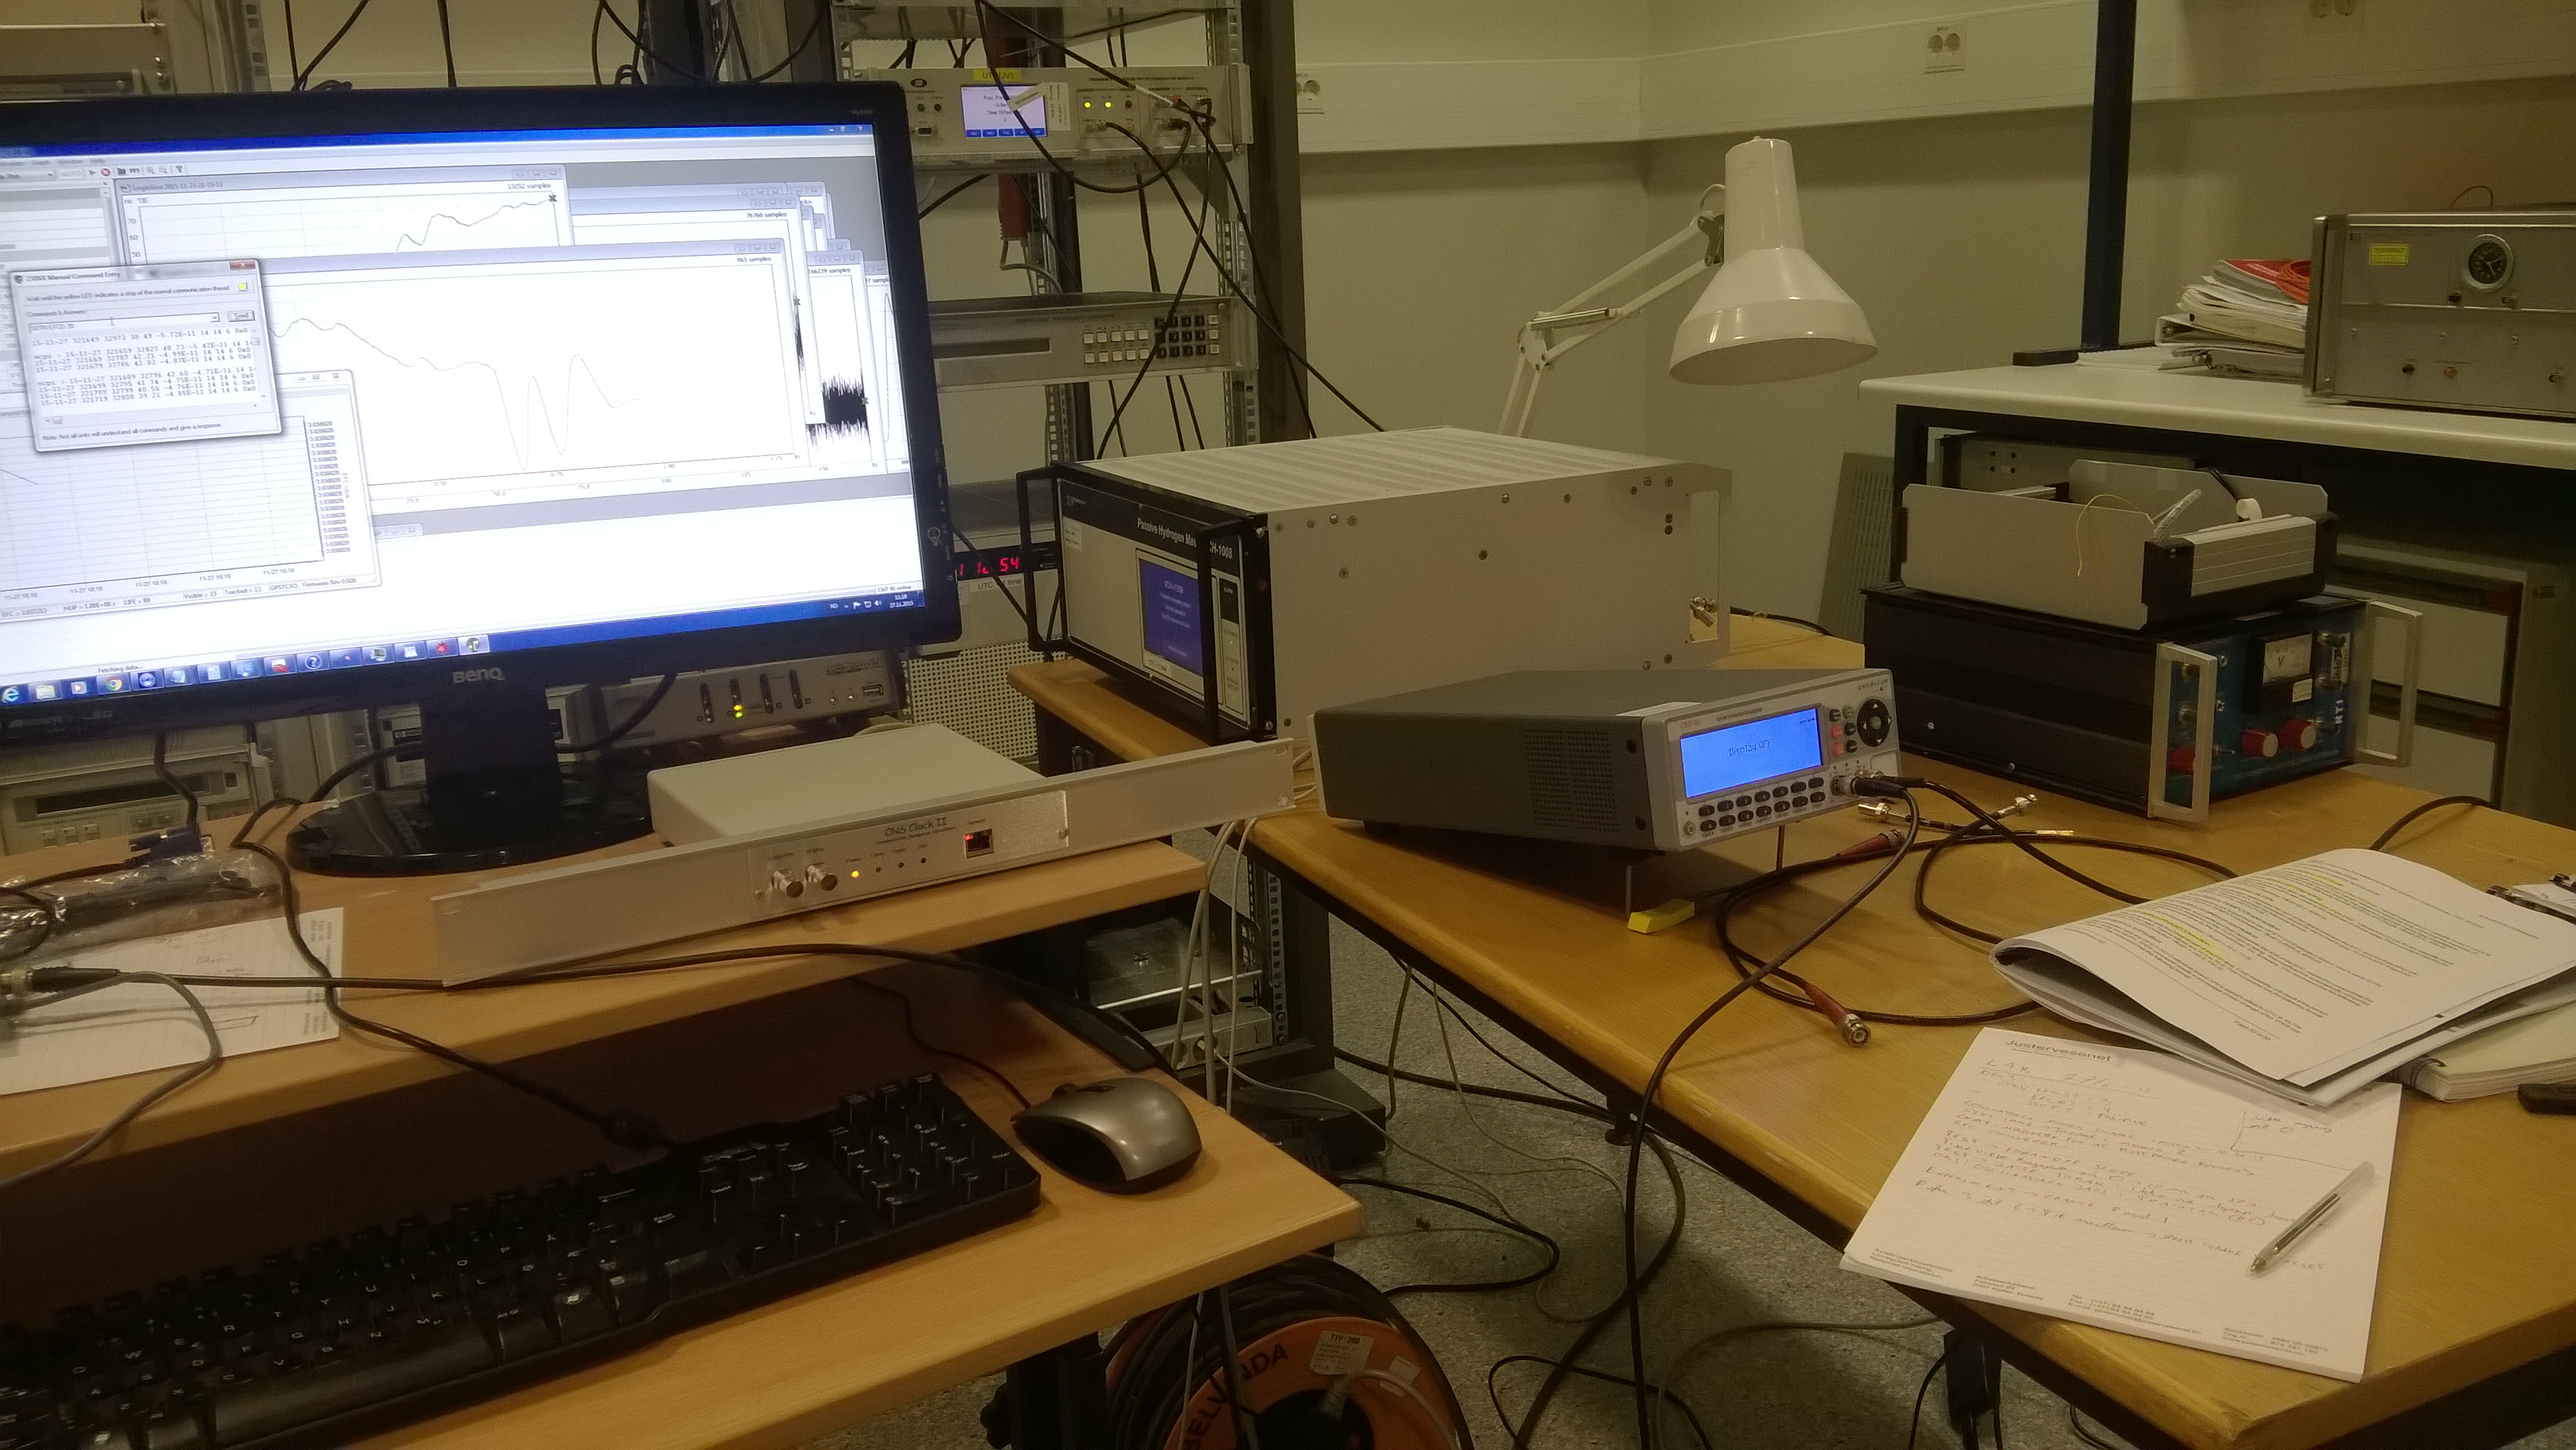
\includegraphics[width=1 \textwidth]{lab.jpg}
\section{Objective}
\begin{itemize}
\item Gain knowledge and understanding of the properties of GPS disciplined oscillator
\item Receive further training in the use of frequency counters as well as tools used to analyze frequency stability.
\end{itemize}

\section{Equipment}
\begin{itemize}
  \item Jackson Labs GPS-300 v1.0 Prototype
  \item Passive Hydrogen maser, frequency reference
  \item Pendulum CNT-91, Frequency counter
  \item Tektronix MD0-4000-6 Oscilloscope
  \item Z38XX Software
  \item TimeView
  \item TimeLab
\end{itemize}

\section{Before the lab}
\begin{itemize}
  \item The GPS-300 was started in advance and had GPS lock for a minimum of 12 hours.
  \item Z3800X was started and configured to store all log data to the applications root folder with the following format for files: \newline \texttt{Z38XX<YEAR>W<WEEK\_NR>.txt}
  \item A TIE measurement was conducted spanning over 10 hours using the CNT-91 as counter with the maser as reference.
\end{itemize}

\section{Part 1: GPS disciplined oscillator}
\begin{wrapfigure}{c}{1\textwidth}
  \centering
  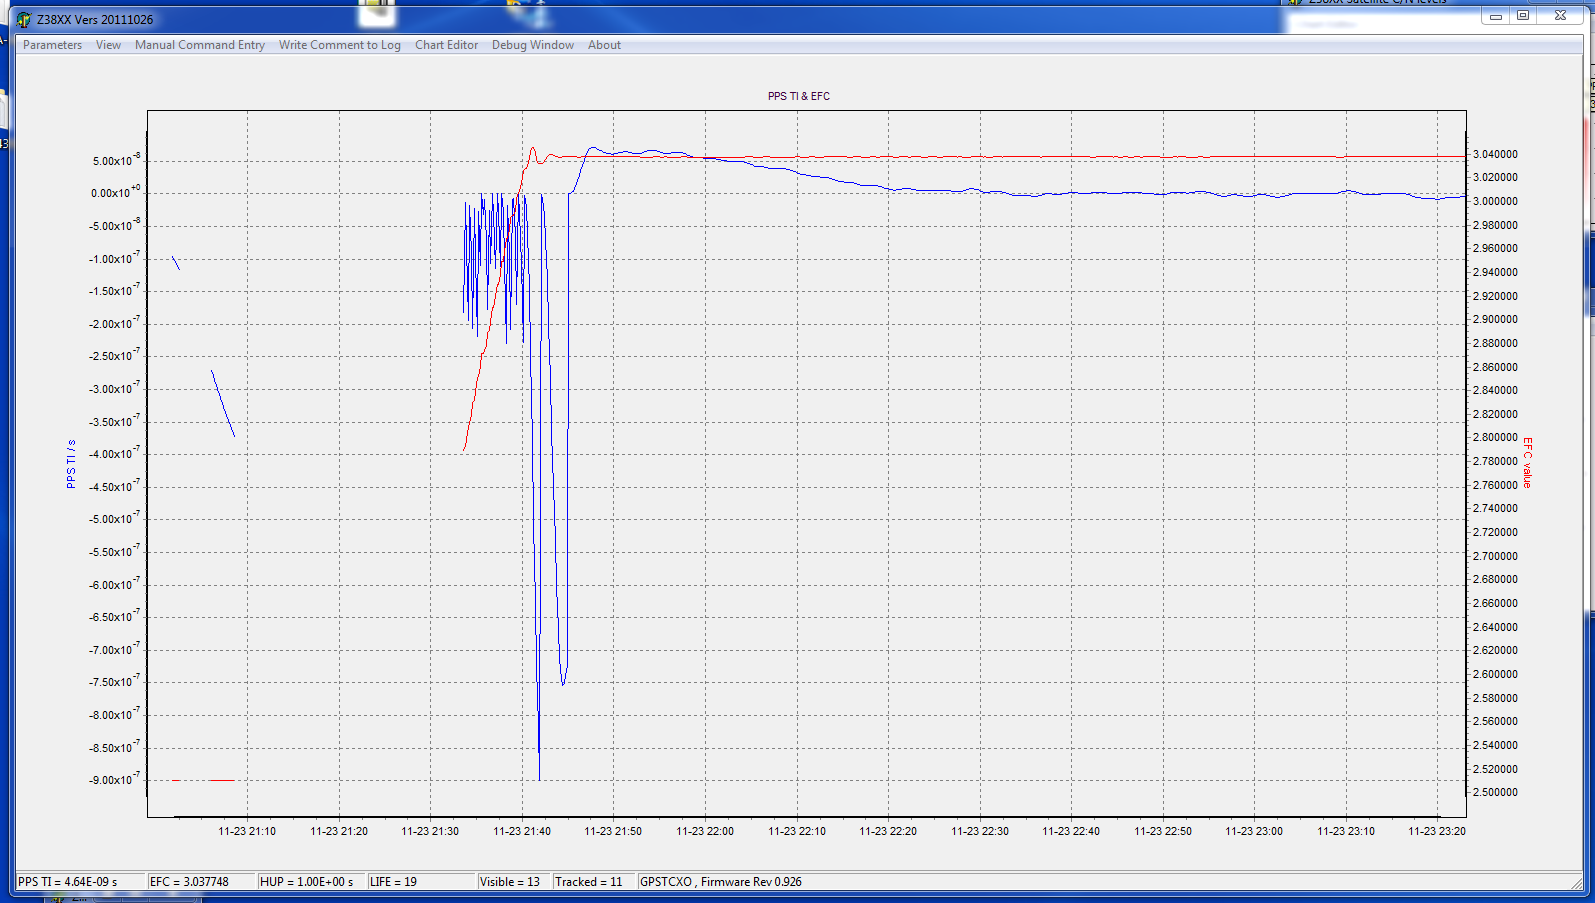
\includegraphics[width=1\textwidth]{z38xx_EFC_oppstart.PNG} \label{fig:z38xx_oppstart}
  \caption[Z38XX screen shot] {The figure above shows a screen shot from the Z38XX software. The oscillator is all warmed up and ready to go.} 
\end{wrapfigure} 
\subsection{Observations}
Figure \ref{fig:z38xx_oppstart} shows that the GPS receiver on the GPS-300 has a total of 13 satellites visible and that it is currently tracking 11, which is more than sufficient for timing purposes. It is also reasonable to assume that it has finished warming up considering how dramatic the readings where and how they are now.

\end{document}                     